\documentclass[11pt]{article}
%Gummi|061|=)
\usepackage[italian]{babel}
\usepackage[utf8x]{inputenc}
\usepackage{hyperref}
\usepackage{graphicx}

\title{}
\author{}
\date{}
\begin{document}

\maketitle

\section{Sviluppo ad alte temperature}

Consideriamo un reticolo quadrato \emph{L}, con \emph{M} segmenti orizzontali e \emph{M} segmenti verticali congiungenti i suoi siti. Queste particolari connessioni, che coinvolgono solo i siti primi vicini, saranno d'ora in avanti chiamate \emph{link}. Nel limite termodinamico in cui $M\to+\infty$, il numero di link $M$ tende al numero di siti $N$ del reticolo, come si può intuire guardando la figura $ \ref{fig1} $, e in particolare i rapporti $\frac{M}{N}$ tra numero di link e di siti.
\begin{figure}[h]
\centering
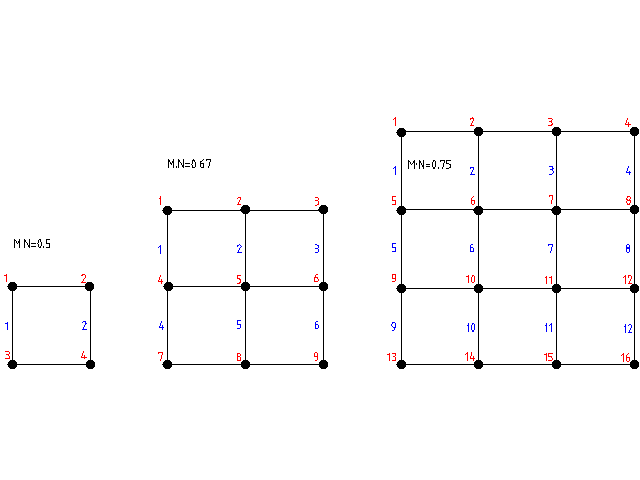
\includegraphics[width=0.72\columnwidth]{sat1}
\caption{tre diversi reticoli}
\label{fig1}
\end{figure}
\\Consideriamo due costanti di accoppiamento $J$ e $J'$ rispettivamente per i link orizzontali e verticali. La funzione di partizione è dunque
\begin{equation} \label{z}
Z_N=\sum_\sigma \exp[K\sum_{(i,j)}\sigma_i\sigma_j+L\sum_{(i,k)}\sigma_i\sigma_k]
\end{equation}
dove $(i,j)$ sono i link orizzontali e $(i,k)$ quelli verticali, mentre $K=\beta J$ e $L=\beta J'$.
Tramite l'identità
$$\exp[x\sigma_i\sigma_j]=\cosh{x}(1+\sigma_i\sigma_j\tanh{x})$$
si può riscrivere $Z_N$ come
\begin{equation}\label{z2}
Z_N=(\cosh{K}\cosh{L})^M\sum_{\sigma}\left(\prod_{(i,j)}(1+v\sigma_i\sigma_j)\prod_{(i,k)}(1+w\sigma_i\sigma_k)\right) 
\end{equation}
dove $v=\tanh{K}$ e $w=\tanh{L}$, sempre $\le1 \ \forall T $. Inoltre per $T\to\infty$ $v$ e $w$ tendono a $0$, e ciò ne giustificherà uno sviluppo in serie.\\
L'argomento tra parentesi tonde nella $\ref{z2}$, risultato del prodotto delle due produttorie, è formato da $2^{2M}$ termini: ogni produttoria è composta da $M$ termini (i link orizzontali o verticali) nella forma $(1+v\sigma_i\sigma_j)$ o $(1+w\sigma_i\sigma_k)$, una volta moltiplicati otteniamo ovviamente un prodotto di $2M$ termini nella stessa forma. Esplicitando il prodotto dei binomi tra parentesi si ottengono i $2^{2M}$ termini cercati, i cui primi termini sono
$$
(1+v\sigma_{1}\sigma_{2})(1+v\sigma_{2}\sigma_{3})...(1+v\sigma_{j}\sigma_{j+1})...(1+w\sigma_{1}\sigma_{2})...(1+v\sigma_{k}\sigma_{k+1})=
$$
$$
1+v\sigma_{1}\sigma_{2}+v\sigma_{2}\sigma_{3}+...+v\sigma_{j}\sigma_{j+1}+...+w\sigma_{1}\sigma_{2}+...+w\sigma_{k}\sigma_{k+1}+...
$$
per passare via via a combinazioni più complesse, la cui generica è
\begin{equation}\label{geomest}
(v\sigma_{\alpha_1}\sigma_{\beta_1})\times... \times (v\sigma_{\alpha_r}\sigma_{\beta_r})\times (w\sigma_{\gamma_1}\sigma_{\delta_1}) \times... \times (w\sigma_{\gamma_s}\sigma_{\delta_s})
\end{equation}
a seconda di quali elementi sto selezionando all'interno del prodotto. I valori estremi che può assumere la $\ref{geomest}$ sono $1$ (se $r=s=0$) e $(vw)^M\sigma_1^4\sigma_2^4\times...\times\sigma_M^4$ (se $r=s=M$). Di sicuro vale $r,s \le M$. \\
 A questo punto possiamo prendere un generico elemento nella forma \ref{geomest} e, per ogni link orizzontale $(v\sigma_{\alpha_i}\sigma_{\beta_i})$ che trovo, lo accendo sul reticolo $L$. Stesso procedimento per i link verticali.\\
 Se ad esempio dei $2^{2M}$ termini scelgo
 \begin{equation}\label{esempioprod}
 (v\sigma_{5}\sigma_{6})(v\sigma_{6}\sigma_{7})(v\sigma_{11}\sigma_{12})(w\sigma_{1}\sigma_{5})(w\sigma_{10}\sigma_{14})
 \end{equation}
 otterrò la figura \ref{confgraf} di sinistra.
 
Un'altra possibile combinazione, che nel capitolo successivo scopriremo essere molto interessante, potrebbe essere
\begin{equation}\label{esempioprodchiuso}
(v\sigma_{1}\sigma_{2})(v\sigma_{5}\sigma_{6})(v\sigma_{6}\sigma_{7})(v\sigma_{10}\sigma_{11})(w\sigma_{1}\sigma_{5})(w\sigma_{2}\sigma_{6})(w\sigma_{6}\sigma_{10})(w\sigma_{7}\sigma_{11})
\end{equation}
a cui corrisponde la configurazione grafica destra in figura \ref{confgraf}.
\begin{figure}
\centering
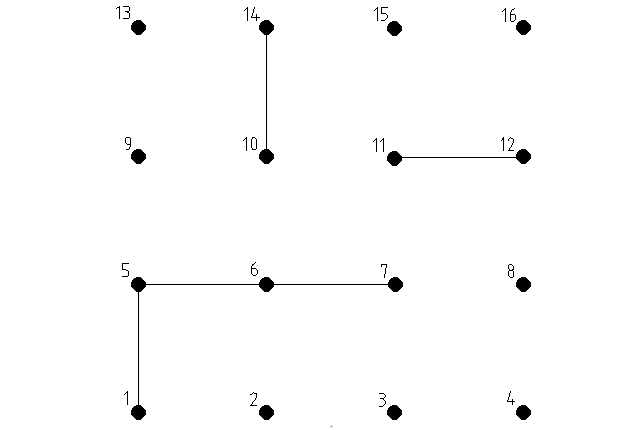
\includegraphics[width=0.47\columnwidth]{sat21}\quad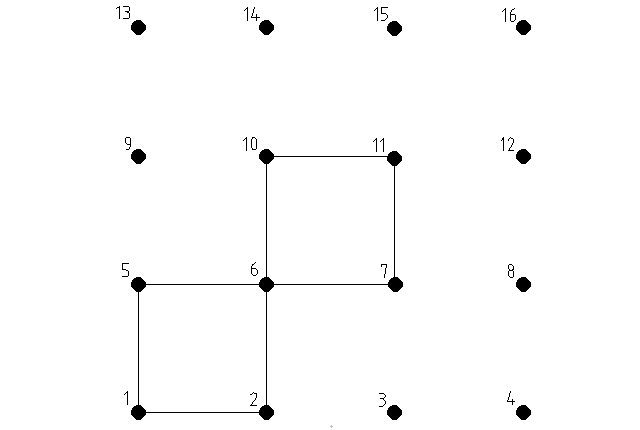
\includegraphics[width=0.47\columnwidth]{sat22}
\caption{configurazioni grafiche sul reticolo della \ref{esempioprod} e della \ref{esempioprodchiuso} }
\label{confgraf}
\end{figure}

 Abbiamo ottenuto un risultato importante, in quanto siamo riusciti ad  assegnare univocamente ad ogni elemento della sommatoria (un oggetto analitico) una configurazione grafica sul reticolo (un oggetto geometrico) e viceversa.
 Ora è anche chiaro perché avevamo introdotto due costanti di accoppiamento $J$ e $J'$.\\
 Possiamo riscrivere questa quantità in maniera più compatta come
\begin{equation}\label{geomcom}
v^rw^s\sigma_1^{n_1}\sigma_2^{n_2}\sigma_3^{n_3}...
\end{equation}
dove $r$ è il numero di link orizzontali accesi, $s$ quelli verticali, e gli $n_i$ il numero di link che partono o finiscono nel sito $i$-esimo. Il prezzo da pagare è che diventa molto più complicato (anche se a rigor di logica sempre possibile) capire come disegnare il grafico associato, in quanto non sappiamo più se un generico $\sigma_{i}$ fosse associato ad un $v$ o un $w$. Sottolineiamo però che questa non è una perdita di informazioni, diventa solo più difficile reperirle.
\\A questo punto non dobbiamo dimenticarci che i termini discussi fin'ora erano in \ref{z2} argomento di una sommatoria  estesa a tutte le configurazioni possibili degli spin sul reticolo, ovvero erano sommati al variare di tutte le possibili combinazioni di valori delle variabili $\sigma_i=\pm1$. Questo implica che se uno o più esponenti $n_i$ fosse dispari, il termine a cui appartengono non sopravvivrebbe nella sommatoria, in quanto verrebbe eliminato dal suo opposto. In altre parole stiamo dicendo che solo i \ $\ref{geomcom}$ \  simmetrici nelle variabili $\sigma_i$ sopravvivono. \\
 L'interpretazione geometrica è che le poligonali devono essere chiuse: non sopravvivono quelle che partono da un punto e arrivano in un altro, perché queste avrebbero $n_i=1$ (o $3$ se ripassa sul punto di partenza lungo il tagitto). Notiamo che è possibile che una configurazione grafica sia formata da più poligonali chiuse disgiunte, nel caso più semplice due quadrati, che però non possono avere un lato in comune. A tal proposito nella figura \ref{confgraf} sopravvivrebbe solo la configurazione di destra. Sul problema delle sovrapposizioni torneremo nel capitolo successivo.\\
Appurato ciò possiamo semplificare ulteriormente la $\ref{geomcom}$ in
\begin{equation}\label{eq:test}
v^rw^s
\end{equation} 
e ne avremo $2^N$ per ogni valore di \emph{r} e \emph{s}.\\
Riscriviamo quindi \ref{z} come
\begin{equation}\label{z3}
Z_N=2^N(\cosh{K}\cosh{L})^M\sum_Pv^rw^s
\end{equation}
con $P$ insieme di tutte le poligonali chiuse che si possono accendere sul reticolo $L$.\\
A parte dei coefficienti (dipendenti dalla temperatura), la funzione di partizione è univocamente determinata dalla quantità
\begin{equation}\label{serie}
\Phi(v,w)=\sum_Pv^rw^s
\end{equation}
Scrivere esplicitamente la \ref{serie} è molto complicato all'aumentare di $r$ e $s$, sia per quanto riguarda il calcolo della degenerazione, sia per il disegnare le configurazioni grafiche associate sul reticolo .\\ 
Se ci accontentiamo di sviluppare $\Phi$ ad alte temperature (quindi nelle variabili $v$ e $w$, che ricordiamo essere piccole ad alte $T$), otteniamo
\begin{equation}
\sum_Pv^rw^s=1+Nv^2w^2+Nv^2w^4+Nv^4w^2+Nv^2w^6+Nv^6w^2+N^2v^4w^4
\label{primiserie}
\end{equation}
Ogni termine ha associata, per quanto discusso prima, una ben definita configurazione grafica ed una degenerazione: vediamone alcune. $1$ corrisponde a non aver tracciato nessun grafico, $(vw)^2$ sono gli $N$ quadrati accendibili sul reticolo, si presentano poi i rettangoli con perimetro di $6$ link con i lati maggiori verticali e orizzontali (anch'essi con degenerazione $N$), idem per quelli da $8$. Il termine $v^4w^4$ porta le configurazioni grafiche di figura \ref{v4w4}. 
\begin{figure}
\centering
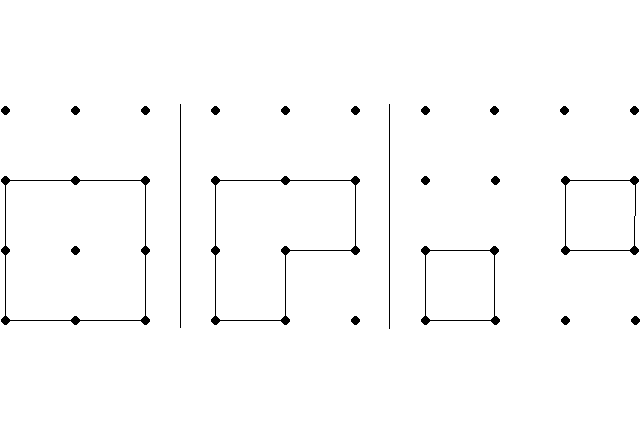
\includegraphics[width=0.9\columnwidth]{sat3}
\caption{configurazioni grafiche sul reticolo di $v^4w^4$ }
\label{v4w4}
\end{figure}
La degenerazione dei quadrati è ovviamente $N$, dei quadrati senza uno spigolo $4N$ ($N$ per ogni tipo), della coppia di quadrati $N(N-5)$, in quanto dopo aver disegnato il primo ho $N-5$ posti dove mettere il secondo. Non posso infatti nè sovrapporlo nè metterlo con dei lati adiacenti. Sommando ottengo il termine $N^2$.





\end{document}
